\documentclass[a4paper, 12pt]{article}

%\usepackage{cmap}
\usepackage[T2A]{fontenc}
\usepackage[utf8]{inputenc}
\usepackage[english, russian]{babel}
\usepackage{graphicx}
\usepackage[top=1in, bottom=1in, left=3.2cm, right=2.6cm]{geometry}
\graphicspath{./}
\usepackage{biblatex}
\addbibresource{lib.bib}
\linespread{1.5}
\usepackage{ragged2e}
\justifying
\usepackage{listings}
\usepackage{color}
\usepackage{amsmath}


\begin{document}
	
\begin{titlepage}
	\fontsize{12pt}{12pt}\selectfont
	\begin{figure}[t!]
		\centering
		
\includegraphics[scale=0.8]{bmstu}
	\end{figure}
	
	\noindent\rule{15cm}{3pt}
	\newline\newline
	\noindent 
	ФАКУЛЬТЕТ 
	\underline{«Информатика и системы управления»} \newline
	
	\noindent КАФЕДРА \underline{«Программное обеспечение ЭВМ и информационные технологии»}\newline\newline\newline\newline\newline
	
	\centering {\Large \textbf{Отчет по лабораторной работе № 3}}
	\vspace{4mm}
	
	\centering {\Large \textbf{По курсу:} Моделирование
		\vspace{8mm}}
	\\ \centering {\Large \textbf{На тему:} Генераторы псевдослучайных чисел}
	\vspace{20mm}
	
	
	\begin{flushright}
		{\small	\textbf{Студент:}\\ Андреев Александр Алексеевич \\ \textbf{Группа:} ИУ7-74Б
			\vspace{3mm}
			\\\textbf{Преподователь:} \\ Рудаков Игорь Владимирович }
	\end{flushright}
	
	\begin{center}
		\vfill
		Москва, \the\year
		~г.
	\end{center}
\end{titlepage}

\tableofcontents
\clearpage
\newpage


\section{{Задание}}

\hspace*{5mm} Изучить и реализовать генератор псевдослучайных чисел программным и табличным методом. Разрядность чисел должна быть равна 1, 2, 3. Сравнить методы по определенному критерию и сделать выводы.

\section{{Теоритическая часть}}
\hspace*{5mm} В данной лаборатоной работе рассматриваются 2 метода генерации случайных чисел:
\begin{enumerate}
	\item программный;
	\item табличный.
\end{enumerate}
\subsection{Программный генератор}
\hspace*{5mm} Программный генератор формирует псевдослучайные числа. Каждое последующее число в такой последовательности зависит от предыдущего.

\subsection{Табличный генератор}
\hspace*{5mm} Табличный генератор использует таблицу проверенных некоррелированных цифр в качестве источника случайных чисел.
\subsection{Критерий случайности}
\hspace*{5mm} Для сравнения описанных методов генерации случайных чисел воспользуемся \textbf{критерием частотности}, который позволяет определить равномерность сгенерированных чисел.

\hspace*{5mm} Определяется количество чисел на интервале $(\mu - \sigma,\ \mu + \sigma)$, где $\mu$~--- математическое ожидание, а $\sigma$~--- среднеквадратичное отклонение. Идеальным результатом будем считать отношение длины рассматриваемого интервала к длине всего промежутка, на котором генерируется последовательность. Под полученным результатом будем понимать отношение количества сгенерированных чисел на интервале к количеству всех сгенерированных чисел.


\section{{Результаты}}
\begin{figure}[h!]
	\centering 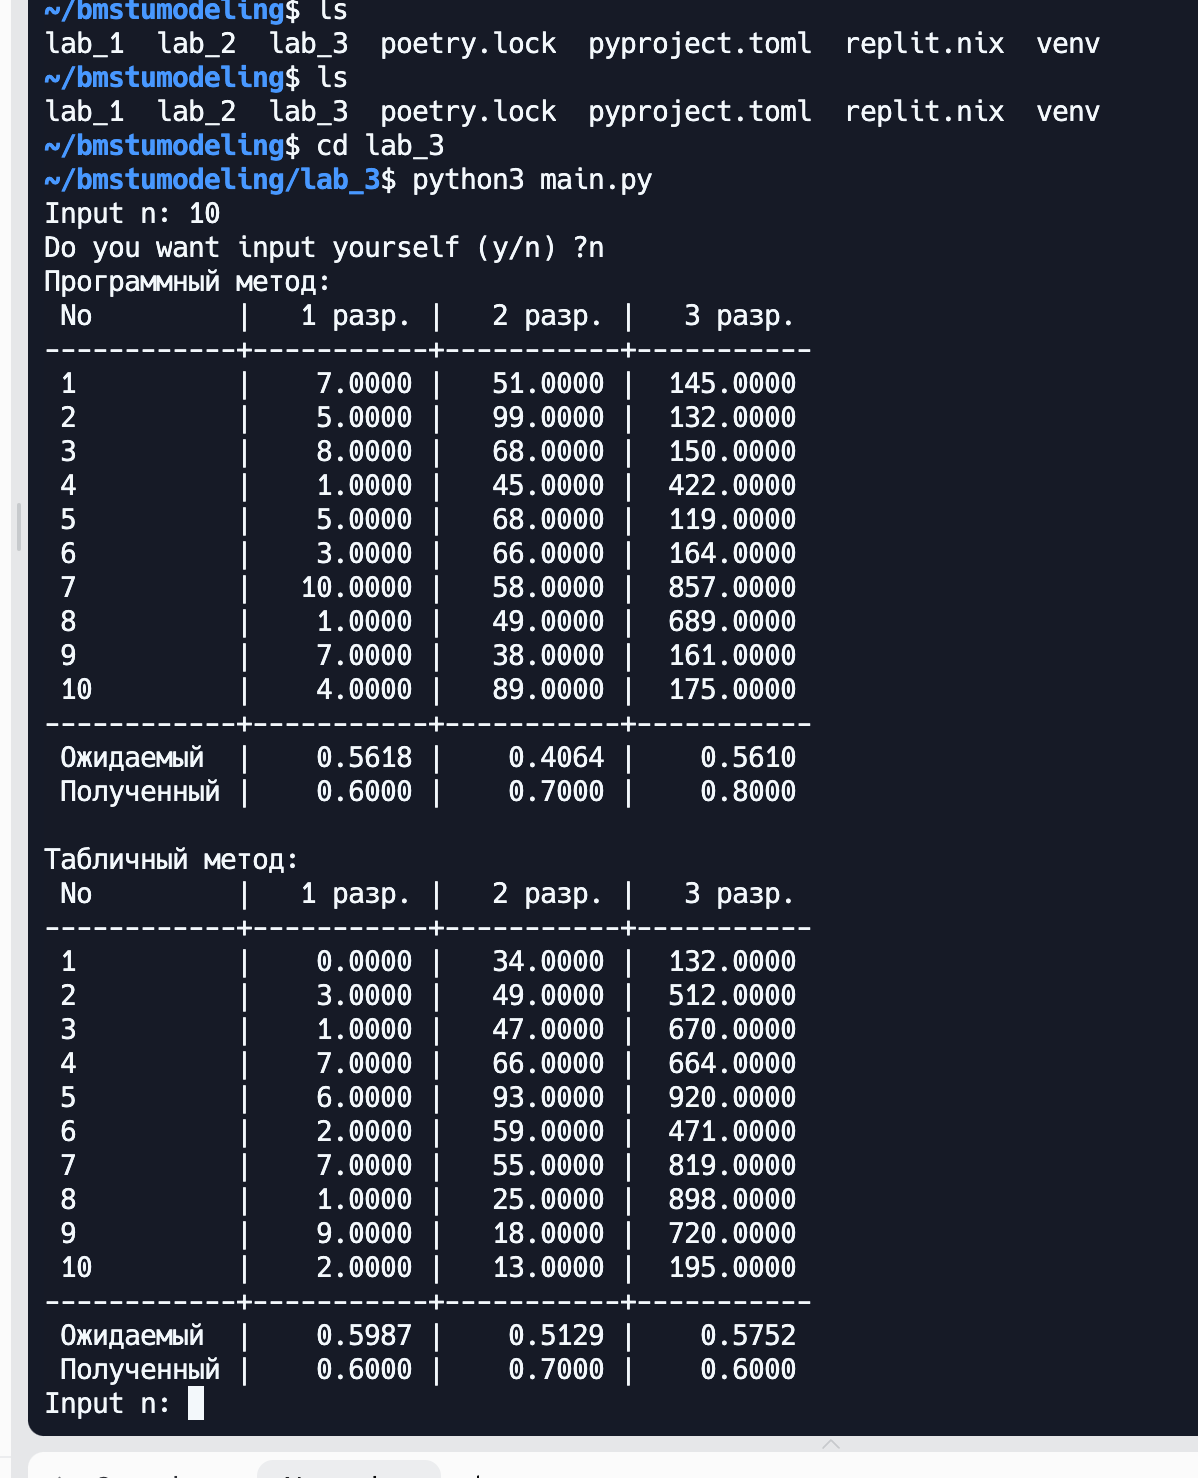
\includegraphics[scale=0.7]{10}
	\centering\caption{Пример работы для 10 чисел}
\end{figure}
\clearpage
\newpage
\begin{figure}[t!]
	\centering 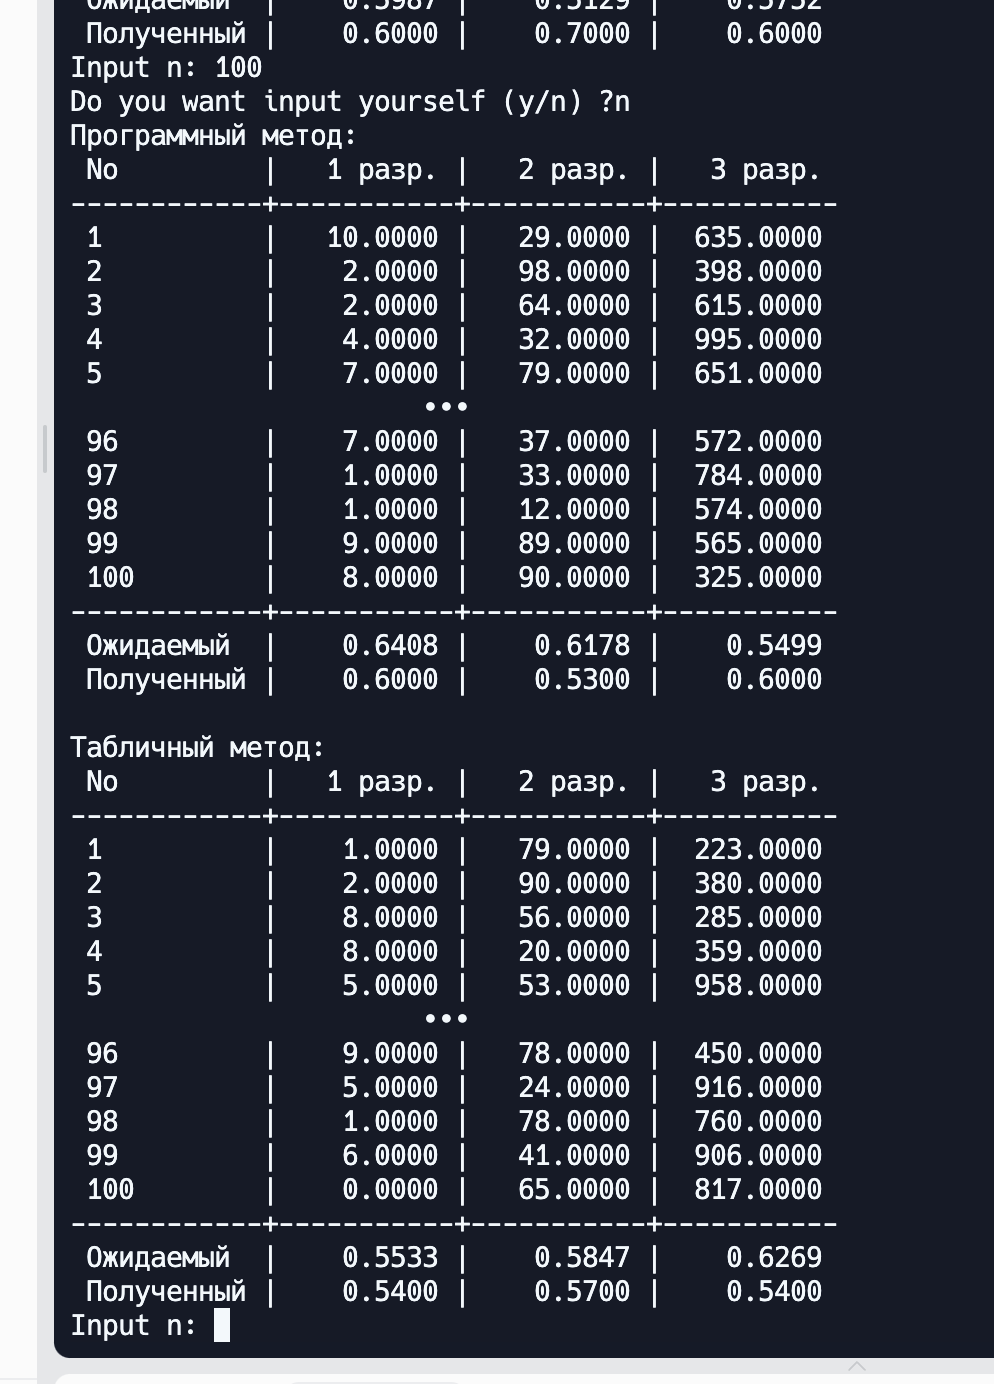
\includegraphics[scale=0.7]{100}
	\centering\caption{Пример работы для 100 чисел}
\end{figure}
\clearpage
\newpage
\begin{figure}[t!]
	\centering 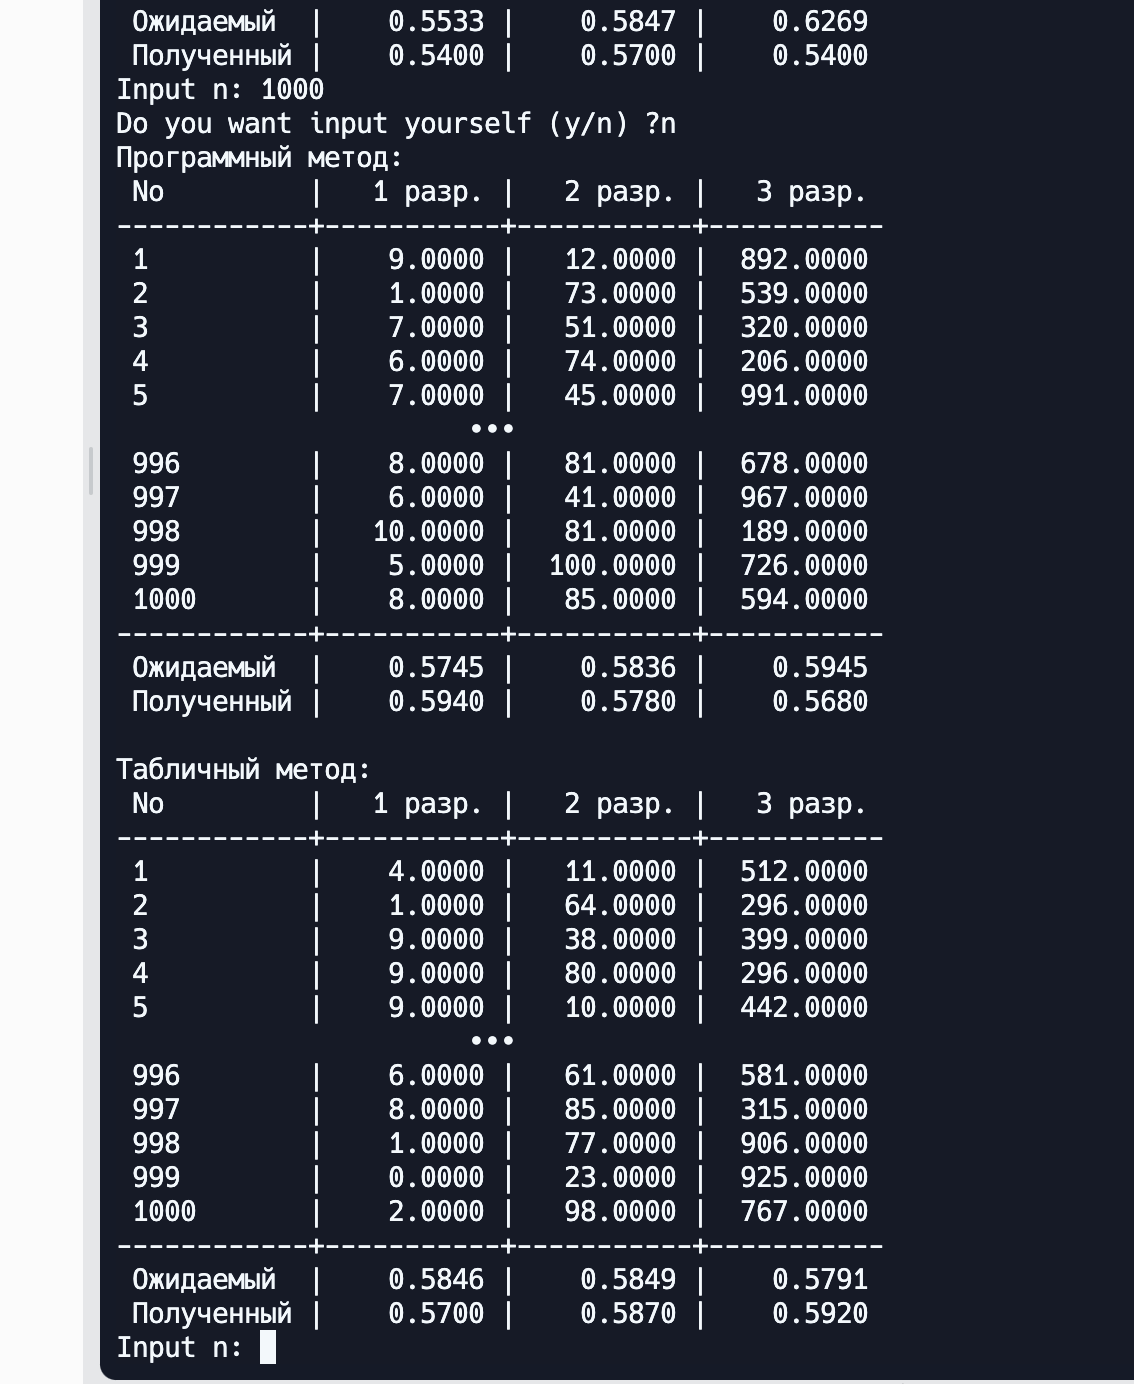
\includegraphics[scale=0.7]{1000}
	\centering\caption{Пример работы для 1000 чисел}
\end{figure}
\clearpage
\newpage
\clearpage
\newpage
\begin{figure}[t!]
	\centering 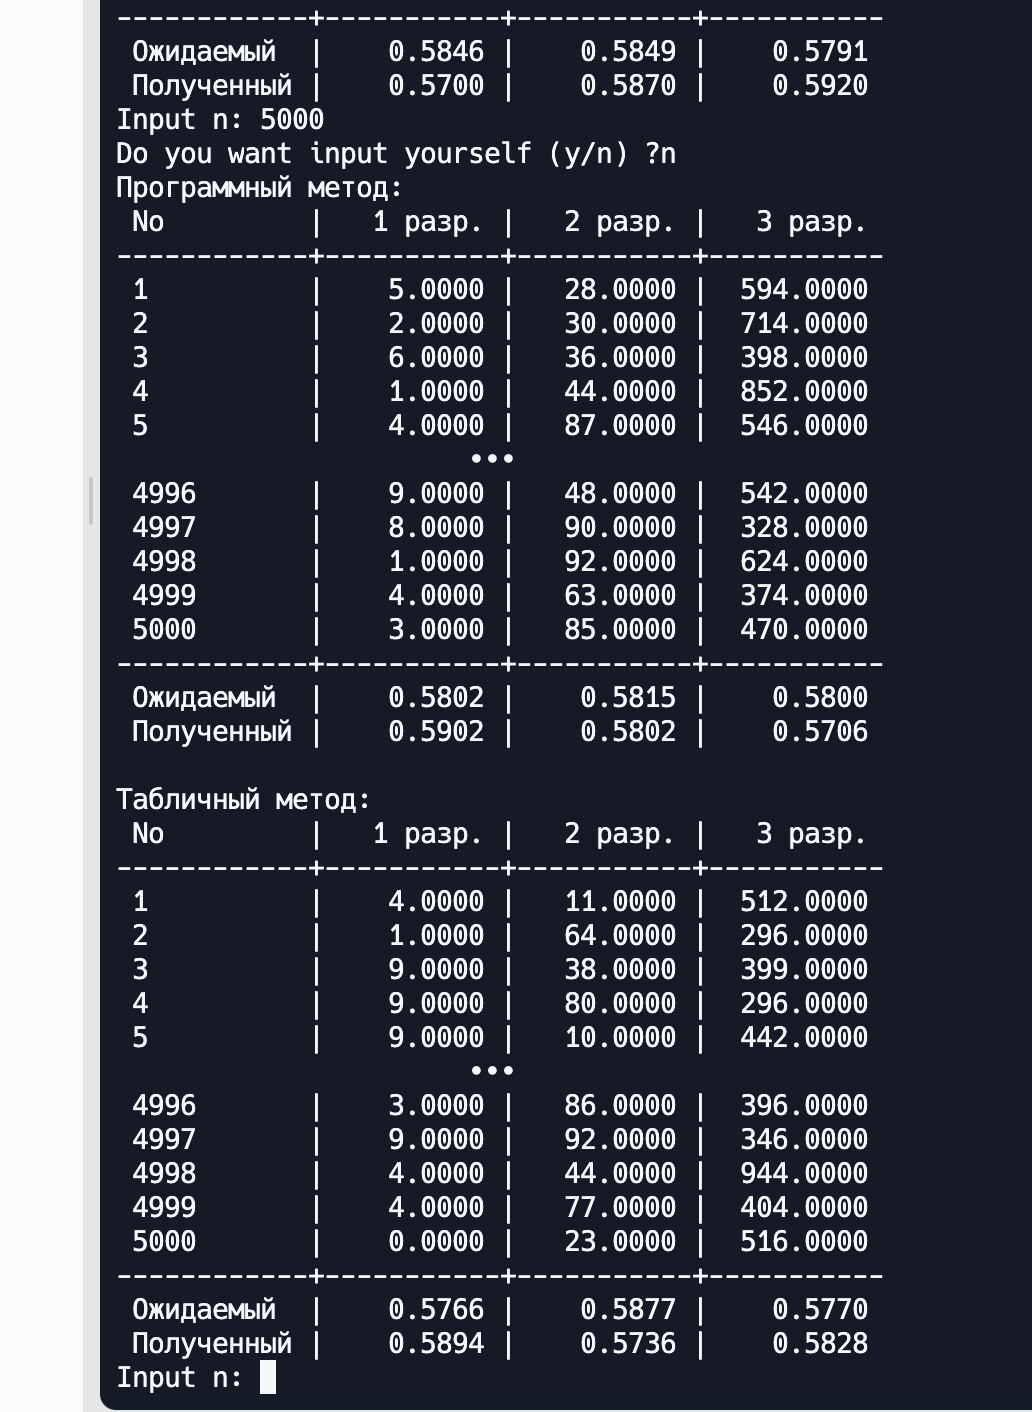
\includegraphics[scale=0.7]{5000}
	\centering\caption{Пример работы для 5000 чисел}
\end{figure}
\clearpage
\newpage
\clearpage
\newpage
\begin{figure}[t!]
	\centering 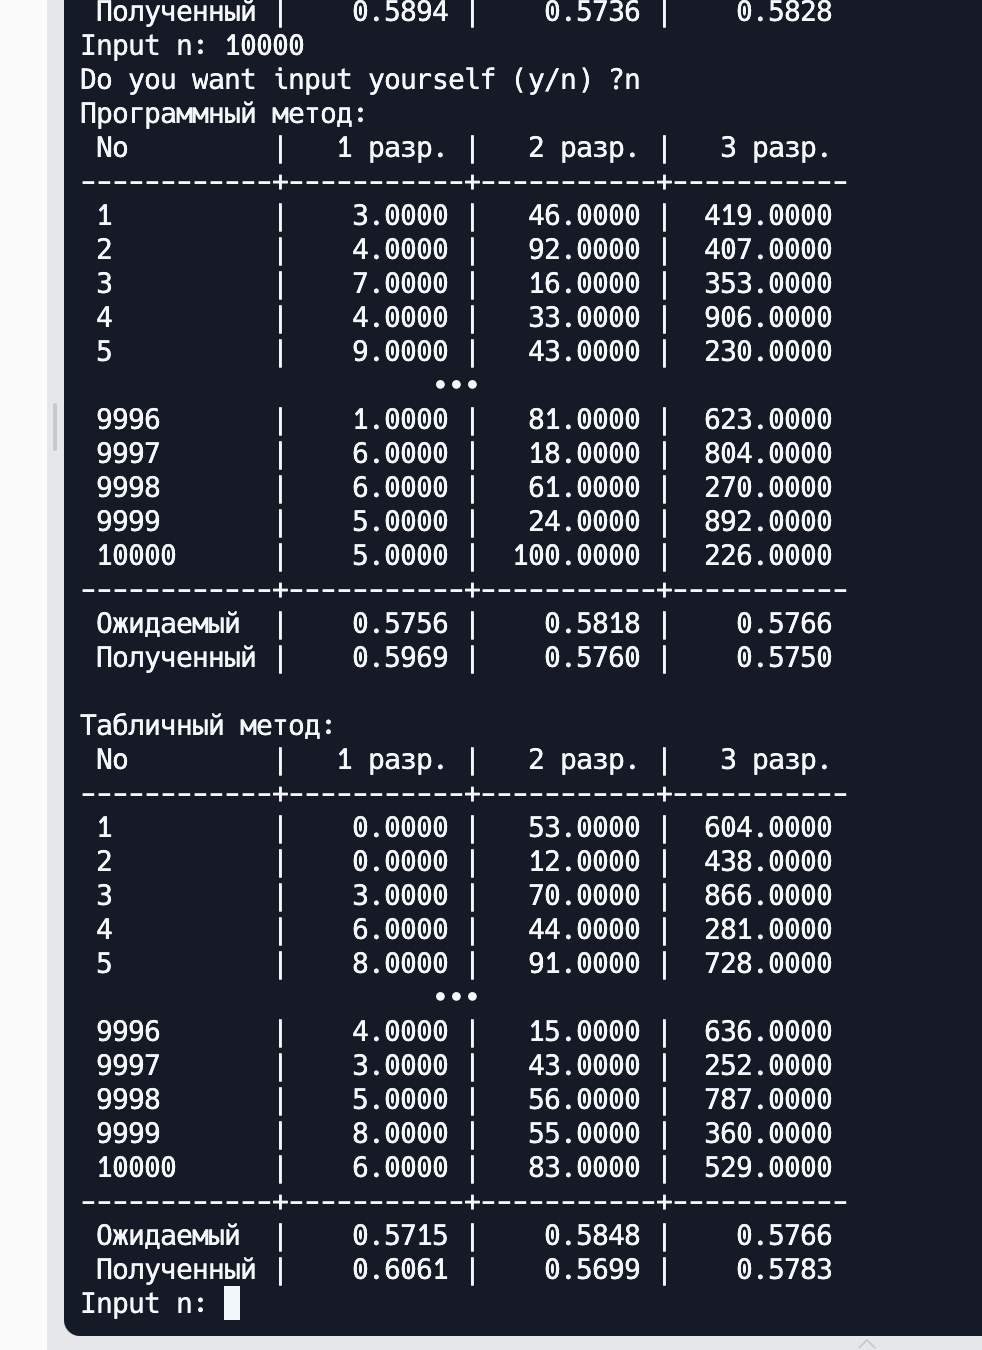
\includegraphics[scale=0.7]{10000}
	\centering\caption{Пример работы для 10000 чисел}
\end{figure}
\clearpage
\newpage
\section{Листинг кода}
\definecolor{codegreen}{rgb}{0,0.6,0}
\definecolor{codegray}{rgb}{0.5,0.5,0.5}
\definecolor{codepurple}{rgb}{0.58,0,0.82}
\definecolor{backcolour}{rgb}{0.95,0.95,0.92}

\lstdefinestyle{mystyle}{
	backgroundcolor=\color{backcolour},   
	commentstyle=\color{codegreen},
	keywordstyle=\color{magenta},
	numberstyle=\tiny\color{codegray},
	stringstyle=\color{codepurple},
	basicstyle=\ttfamily\footnotesize,
	breakatwhitespace=false,         
	breaklines=false,                 
	captionpos=b,                    
	keepspaces=true,                 
	numbers=left,                    
	numbersep=5pt,                  
	showspaces=false,                
	showstringspaces=false,
	showtabs=false,                  
	tabsize=4
}

\lstset{style=mystyle}

\begin{lstlisting}[language=Python, caption = Корневая часть (main.py)]
from io_operations import *
from logics import *


def main():
  # Initializing cicling counting
  while True:
    # Getting starting args
    number, mode = IO_operations().get_args()

    # Getting lists
    slists, tlists = Logics.get_lists(number, mode)

    # Output data
    IO_operations().out_data(number, slists, tlists)

if __name__ == "__main__":
  main()
\end{lstlisting}

\begin{lstlisting}[language=Python, caption = Основная логическая часть (logics.py)]
from my_random import *


# Loginc operator
class Logics():

  def get_lists(n, mode):
    slists = [[], [], []]
    tlists = [[], [], []]

    # Programm input
    if mode == "n":
      sgen = StandardRandom()
      tgen = TableRandom()
      for i in range(n):
        for j in range(3):
          slists[j].append(sgen.get(j + 1))
          tlists[j].append(tgen.get(j + 1))
    # Manual input
    elif mode == "y":
      for i in range(n):
        for j in range(3):
          print("Input ", j + 1, "bitness number:")
          num = float(input())
          slists[j].append(num)
          tlists[j].append(num)

    return slists, tlists
\end{lstlisting}

\begin{lstlisting}[language=Python, caption = Работа с вводом и выводом в терминале (io_operaions.py)]
import tabulate
import numpy
import sys


class IO_operations():
  # Getting starting args
  def get_args(self):
    return int(input("Input n: ")), input("Do you want input yourself (y/n) ?")

  # Output data
  def out_data(self, n, slists, tlists):
    print("Программный метод:")
    self.__print_table(self.__create_table(slists), n)
    print()

    print("Табличный метод:")
    self.__print_table(self.__create_table(tlists), n)

  # Creating table
  def __create_table(self, sequences: list) -> str:
    cols = [list(range(1, len(sequences[0]) + 1))]

    for seq in sequences:
      cols.append(seq.copy())

    cols[0] += ['Ожидаемый', 'Полученный']

    for i in range(1, len(cols)):
      cols[i] += list(self.__frequency_criterion(cols[i], i))

    table = tabulate.tabulate(
      {
        "No": cols[0],
        "1 разр.": cols[1],
        "2 разр.": cols[2],
        "3 разр.": cols[3],
      },
      headers="keys",
      tablefmt="presto",
      numalign="right",
      floatfmt=".4f")

    return table

  # Outputing table with formting with special symbols
  def __print_table(self, table, n):
    rows = table.split('\n')
    print('\n'.join(rows[:5 + 2]))
    if n > 10:
      print(("{:^%ds}" % len(rows[0])).format('\u2022' * 3))
    print('\n'.join(rows[-5 - 2:-2]))
    print(rows[1])
    print('\n'.join(rows[-2:]))

  # Getting frequency 
  def __frequency_criterion(self, sequence, num_len):
    mean = numpy.mean(sequence)
    stdd = numpy.sqrt(numpy.var(sequence))

    cnt = 0
    for item in sequence:
      if (mean - stdd) < item < (mean + stdd):
        cnt += 1

    sequence_max_delta = 10
    if num_len > 1:
      sequence_max_delta = 9 * 10**(num_len - 1)

    return (2 * stdd / sequence_max_delta), (cnt / len(sequence))
\end{lstlisting}

\begin{lstlisting}[language=Python, caption = Программная реализация генерации псевдослучайных чисел программным и табличным методом (my_random.py)]
import random
import datetime


# Obj.__name__ of lib. rand
class StandardRandom():

  def get(self, num_len: int):
    return random.randint(10**(num_len - 1), 10**num_len)


# Obj. of table rand.
class TableRandom():

  def __init__(self, path_to_table: str = "./table.txt"):
    self.digits = ""

    with open(path_to_table) as table_file:
      for line in table_file:
        self.digits += line[:-1]

    self.idx_init()

  # Steping timing
  def idx_step(self, step: int = 1):
    self.idx += step

    if self.idx + step >= len(self.digits):
      self.idx_init(step)

  # Initing timing
  def idx_init(self, offset: int = 0):
    now = datetime.datetime.now()
    self.idx = int((now.microsecond % 60) / 60 \
    * (len(self.digits) - offset))

  def get(self, num_len: int):
    self.idx_step(num_len)
    rnd_num = int(self.digits[self.idx:self.idx + num_len])

    while len(str(rnd_num)) < num_len:
      self.idx_step()
      rnd_num = rnd_num * 10 + int(self.digits[self.idx])

    return rnd_num
\end{lstlisting}
\section{Вывод}
\hspace*{5mm} В результате проведенной лабораторной работы оказалось видно, что при увеличении числа генерируемых случайных чисел, увеличивается равномерность их распределения.
\end{document}